%!TEX root = ../thesis.tex
%*******************************************************************************
%****************************** Third Chapter **********************************
%*******************************************************************************
\chapter{Diseño Conceptual}

% **************************** Define Graphics Path **************************
\ifpdf
    \graphicspath{{Chapter3/Figuras/}{Chapter3/Figs/PDF/}{Chapter3/Figs/}}
\else
    \graphicspath{{Chapter3/Figs/Vector/}{Chapter3/Figs/}}
\fi

\section{Requerimientos del sistema}
Uno de los requerimientos principales del sistema es el uso de una red de sensores modular y sencilla de instalar en distintos tipos de vehículos. Esto se explica fácilmente debido a que este sistema esta orientado a ser usado en el sistema de transporte público en Lima, el cual tiene una gran variedad y un gran número de vehículos. El sistema, entonces, debe ser adaptable a cualquiera de estos vehículos y no contar con un tiempo de instalación elevado.

También se tiene como requerimiento un grado de precisión alto en el reconocimiento de estilos y eventos de conducción. Esto es necesario debido a que este sistema se usará para monitorizar y mejorar la conducta de conducción de los choferes del servicio de transporte público. Los datos arrojados por este sistema necesitan ser confiables.

Por último, se necesita también de una adecuada infraestructura que permita que el sistema funcione en linea, entregando feedback al conductor, aún si se presentan condiciones como la falta temporal de conexión a Internet. Este requerimiento será importante al considerar donde realizar el procesamiento de los datos (dentro de un sistema embebido en cada vehículo o usando un servidor).

% Please add the following required packages to your document preamble:
% \usepackage{multirow}
\begin{table}[htbp!]
  \caption{Lista de Requerimientos página 1}
  \label{diag:2.1}
  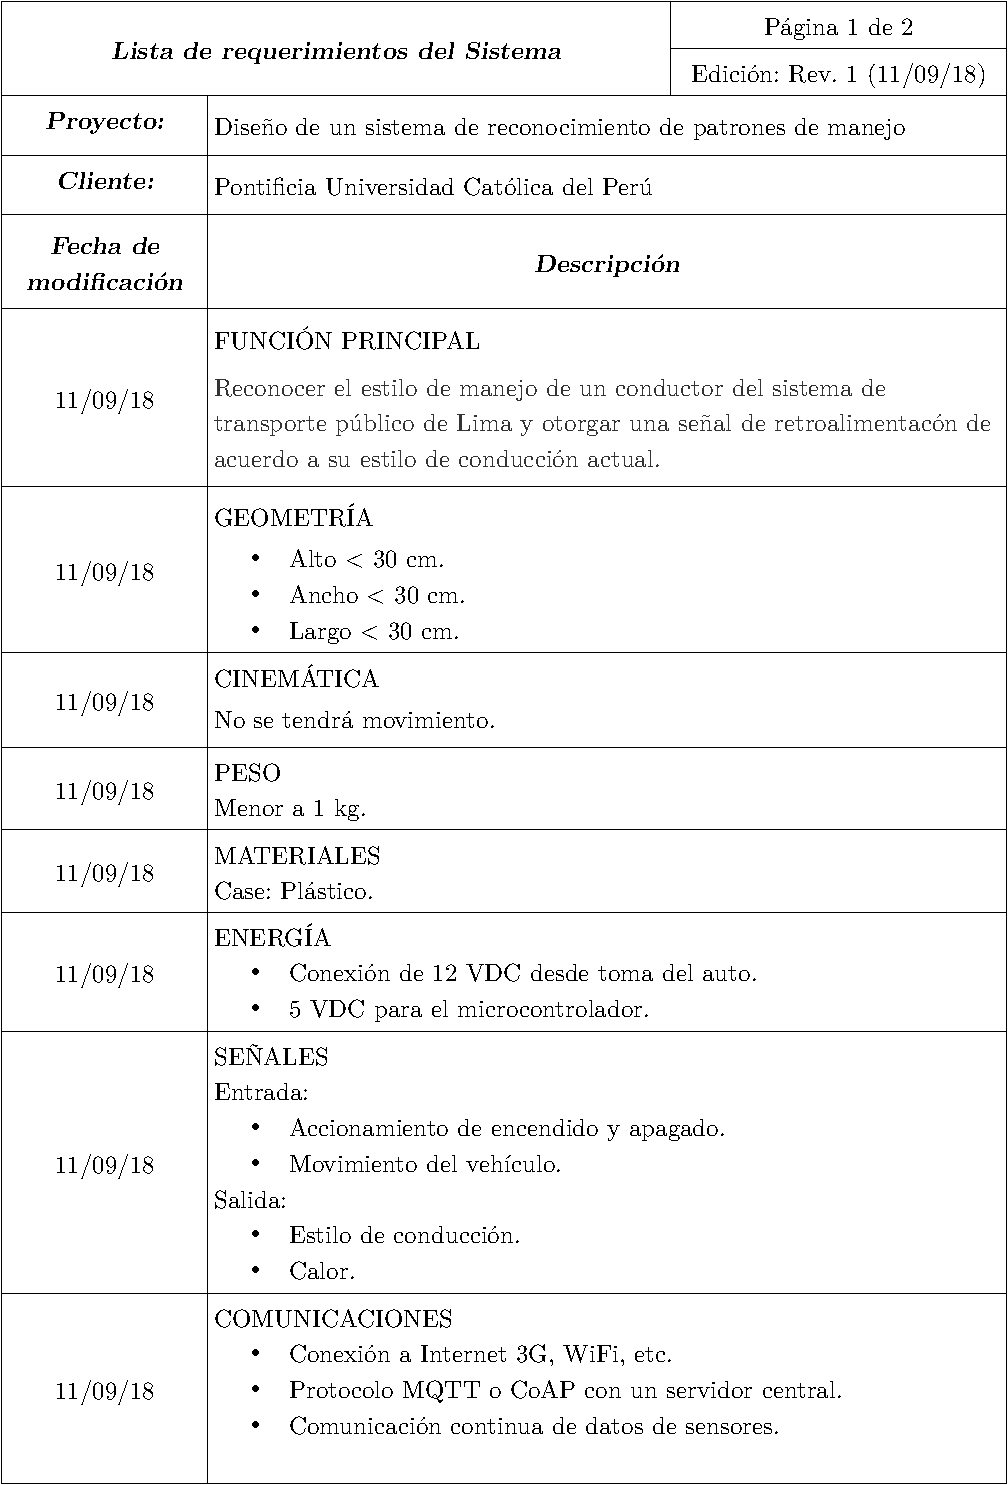
\includegraphics[width=1.05\linewidth]{Tab1.pdf}
\end{table}

\newpage

\begin{table}[htbp!]
  \caption{Lista de Requerimientos página 2}
  \label{diag:2.2}
  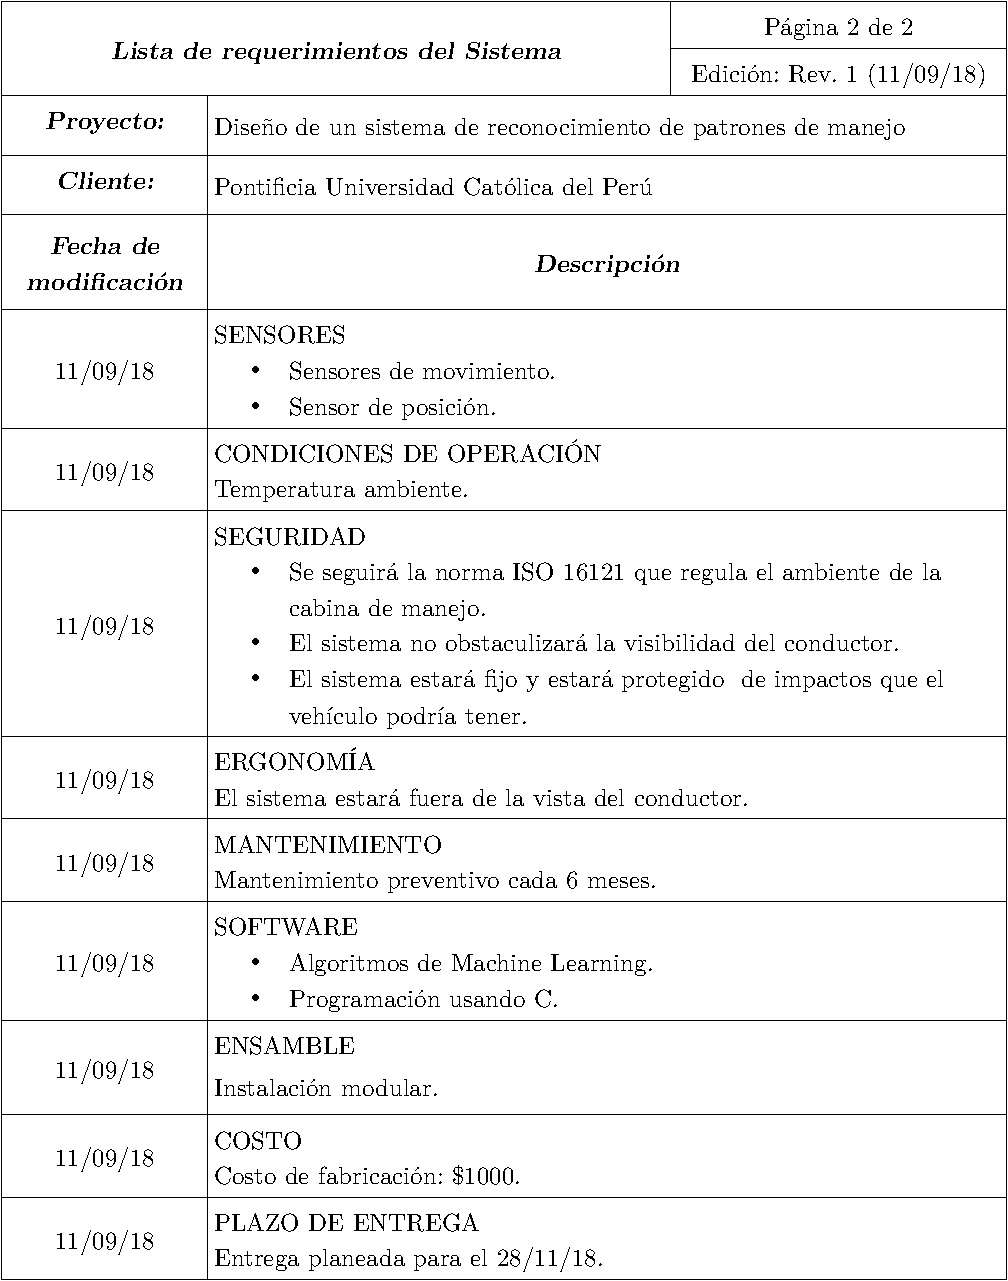
\includegraphics[width=1.05\linewidth]{Tab2.pdf}
\end{table}

\section{Modelo Black Box}
En la Fig~\ref{fig:3.1} se puede observar el modelo de Black Box o Caja Negra del sistema. En este modelo se pueden apreciar con mayor claridad las entradas y salidas del sistema

\begin{figure}[htbp!]
\centering
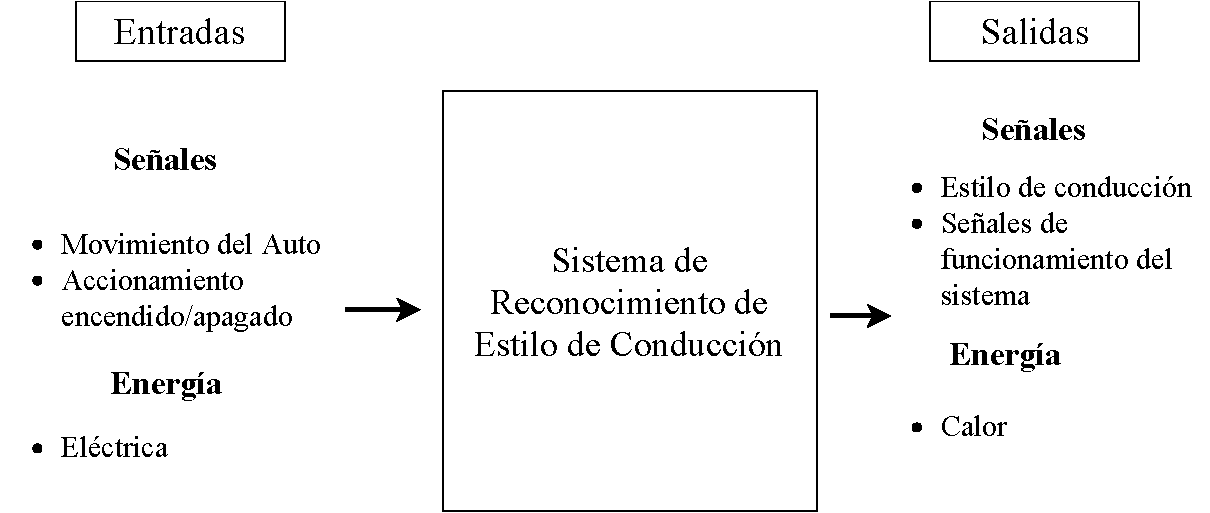
\includegraphics[width=\textwidth]{Fig1.pdf}
\caption{Modelo de Black Box del sistema}
\label{fig:3.1}
\end{figure}


El sistema estará conectado al auto, de donde obtendrá la energía necesaria para funcionar. Debido a que el enfoque del sistema es ahorrar energía. Su consumo debe ser reducido.

Además de recibir la energía, este sistema procesará el movimiento del auto usando sensores obteniendo así toda la información necesaria para caracterizar el estilo de conducción del usuario. El estilo de conducción será almacenado y será representado como una señal de feedback al usuario. Además el sistema deberá indicar al usuario que se en funcionamiento.

\section{Estructura de Funciones}

\begin{sidewaysfigure}[htbp!]
\centering
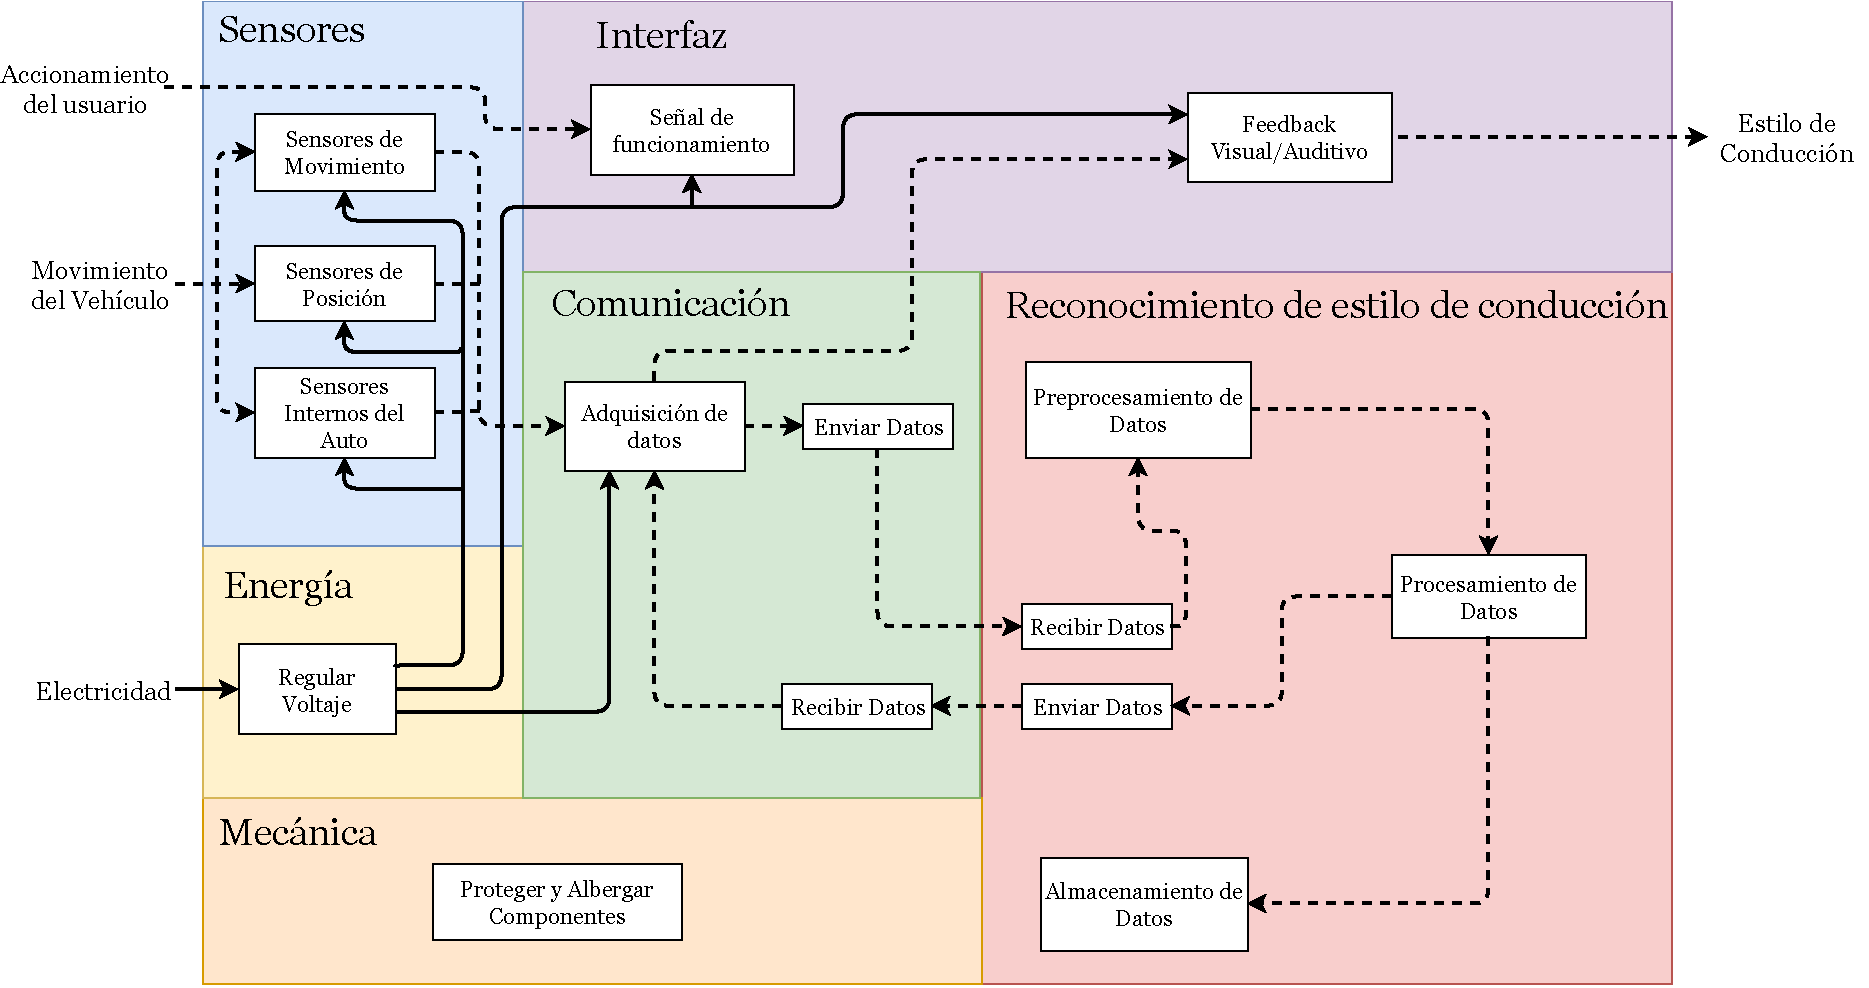
\includegraphics[width=\textwidth]{Tab3.pdf}
\caption{Estructura de Funciones}
\label{fig:3.2}
\end{sidewaysfigure}

La estructura de funciones del sistema se puede apreciar en la Fig~\ref{fig:3.2}. Para el elaboramiento de esta se han considerado 5 módulos: Energía, Mecánica, Sensores, Comunicación y Reconocimiento del estilo de conducción.

Se describirá a continuación cada uno de estos módulos para así obtener una visión general del funcionamiento total del sistema.

\subsection{Módulo de energía}
En este módulo se maneja la energía eléctrica que alimenta al sistema. Esta es obtenida directamente del automóvil (Conexión de \SI{12}{V}) y transformada según los requerimientos de los sensores y módulos que van conectados al microcontrolador (MCU). Estos requerimientos normalmente pueden ser de \SI{3.3}{V} o \SI{5}{V} y de un amperaje menor a \SI{1}{A}.

Este módulo también energiza al dispositivo de feedback al usuario, que podría ser una pantalla y/o unos parlantes. Estos se encuentran en un rango de potencia similar a la mencionada anteriormente.

\subsection{Módulo mecánico}
En este módulo se encuentra la estructura que se encargará de sostener y mantener seguros a todos los componentes electrónicos del sistema. Debido a que el auto en el que el sistema estará instalado se desplazará y estará sujeto a aceleraciones, es necesario que esta estructura mantenga inmóvil al sistema con respecto al vehículo.

\subsection{Módulo de sensores}

Este módulo se encarga de transformar el movimiento del vehículo en información útil para poder caracterizar el estilo de conducción del usuario. Esta compuesto por sensores inerciales, un módulo GPS y los sensores de los {\it Electronic Control Units} (ECU) del vehículo, si se encuentran disponibles.

Todos estos elementos se encontrarán enviando información constantemente al MCU para que este la maneje.

\subsection{Módulo de comunicación}
Este módulo se encargará de encender una señal que indique que el sistema se encuentra en funcionamiento y también de enviar los datos que fueron entregados por el módulo de sensores hacia un servidor. Esto se logrará usando un módulo 3G y empleando un protocolo que permita enviar información a una velocidad adecuada y sin requerir mucho poder de procesamiento, como MQTT o CoAP.

Además este módulo recibirá a través del servidor el resultado del procesamiento de los datos que envió. Este resultado es el estilo de conducción actual del usuario. El microcontrolador mostrará esta información al usuario usando una interfaz audiovisual, como una tablet o pantalla, a forma de feedback de su actividad de conducción.

\subsection{Módulo de reconocimiento de estilo de conducción}
En este módulo se realizará el procesamiento de la data que fue enviada por el MCU. Para realizar esto se realizará un preprocesamiento de la data para luego procesarla usando algoritmos de machine learning.

Cuando la data haya sido procesada, se tendrá el estilo de conducción resultante que será enviado de vuelta al MCU por el servidor. Sin embargo, la data usada para obtener este resultado se conservará. Esta data se almacenará en el servidor para poder hacer análisis offline o implementar otros servicios que puedan hacer uso de la información disponible, como un seguimiento en tiempo real de los buses, un monitoreo de los conductores, etc.
